Visuomotor policies are increasingly trained from camera observations rather than hand-designed state estimates. This shift makes the camera setup part of the learning problem. A policy trained under one camera distribution can be evaluated under another, and deployment cameras may be moved, replaced, or unavailable as calibrated sensors. Standard image policies avoid explicit calibration, but they may solve the training distribution through view-specific correlations rather than through camera-aware reasoning.

Geometry-aware alternatives typically inject calibrated camera poses, rays, depth, point clouds, or reconstructed 3D state into the policy. These approaches add useful inductive bias, but they also move part of the system outside the learned control objective. A calibrated pose may be geometrically correct yet not optimally aligned with the representation used by the policy. Separate reconstruction or pose-estimation stages can also introduce dependencies that are hard to satisfy in large-scale robot data.

This work studies camera geometry as an end-to-end learning problem for control. We ask whether camera pose prediction can be trained jointly with imitation learning, using only partial pose labels as an auxiliary signal, and whether action loss can shape the learned geometry toward task-relevant control. We further study a view-synthesis variant in which held-out target views are reconstructed from latent observation tokens, imposing a renderability constraint on the encoder during training.

The paper evaluates two model variants. The first is an end-to-end camera-pose action policy: observations are passed to a camera-pose predictor, pose or ray tokens condition an observation encoder, and an action expert predicts action chunks. The second adds novel-view synthesis: a register-style observation encoder feeds both the action expert and an NVS decoder queried by target camera pose. The two variants are separate model instantiations rather than one shared encoder with an optional head.

Our current evidence comes from two settings. LIBERO-MV Spatial tests whether partial camera-pose supervision is enough for end-to-end pose-policy learning. MimicGen camera-shift evaluation tests whether NVS regularization improves robustness when the evaluation cameras differ from the training camera distribution.

\begin{figure}[t]
  \centering
  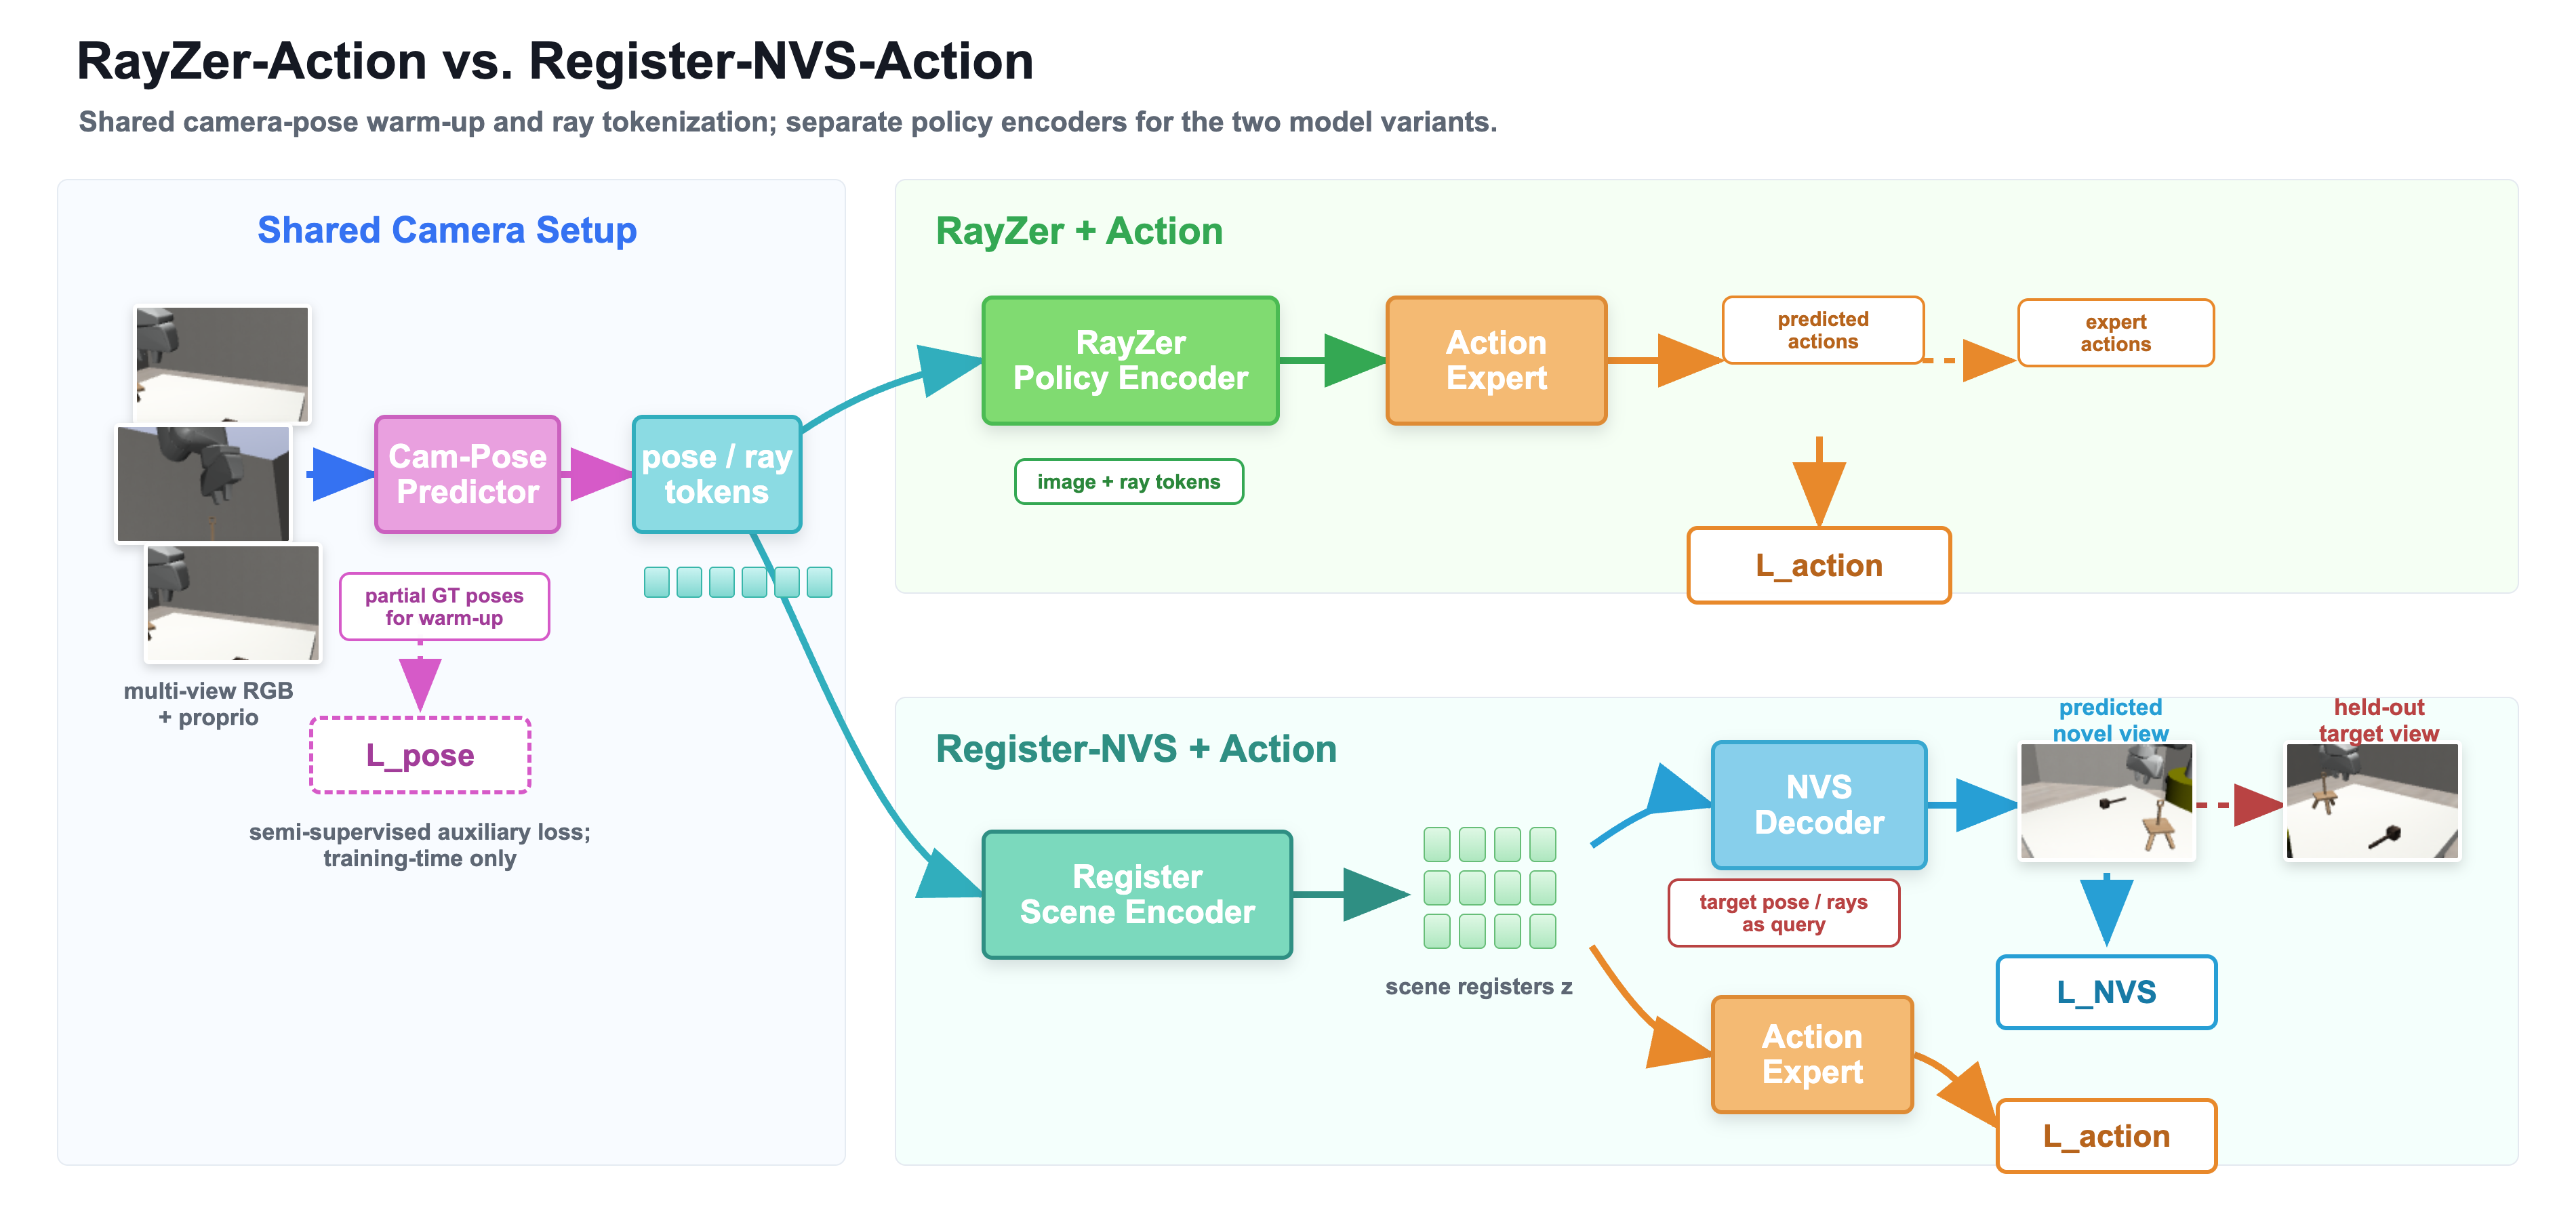
\includegraphics[width=\linewidth]{figures/pipeline.png}
  \caption{Draft pipeline figure. The camera-pose predictor and ray-tokenization stage are shared in the setup, but RayZer-style action training and register-token NVS training use separate observation encoders.}
  \label{fig:pipeline}
\end{figure}
